\section{Evaluation}
\labsection{evaluation}


In this Section, we evaluate the implementation of the algorithm
described in \refsection{stm}.  
We implemented our algorithm in the context of \textsc{TinySTM}~\cite{FelberFMR10}, which we also use as baseline for our evaluation. %and we compare this implementation with the vanilla \textsc{TinySTM}.
The experiments are conducted on an AMD Opteron48, a 48-cores machine with 256 GB of RAM. 
This machine embeds 4 dodeca-core AMD Opteron 6172, and 8 NUMA nodes.

To evaluate the performance our implementation, we use the test suite included with \textsc{TinySTM}. 
This test suite is composed of several STM applications with different transaction patterns.
The reminder of this section briefly describes the benchmarks as well discussing our results.
 
\subsection{Benchmark: Bank}

The bank benchmark consists in simulating transfers between bank accounts. 
Each transaction reads two accounts and updates the two accounts. 
We run this benchmark with 10k bank accounts, and a locality
of 0.8 (meaning that 80\% of transfers are local to a thread, while 20
\% are between any account). 
We measure the number of transfers performed by a set of threads in 10 seconds.
The results are reported in Figure~\ref{fig:benchmarking:bank}.%\ft{todo: include a  figure showing the performance (with locality=0.8 ?)}
%
The results show that the performance obtained with the global clock
merely improve as the number of thread increases: 48 threads achieve 2.8
millions transactions per second, while 1 thread achieve 2.2 millions
transactions per second.
%
Our implementation perform better: the speedup obtained with 48 threads reaches 3100 \%. 
Figure~\ref{fig:benchmarking:bank:speedup} shows the speedup for different levels of locality.
This  can be explained by the low contention in this application: since the threads each work on independant data, there is no contention when  performing the transactions.

\begin{figure}[!t]
	\centering
	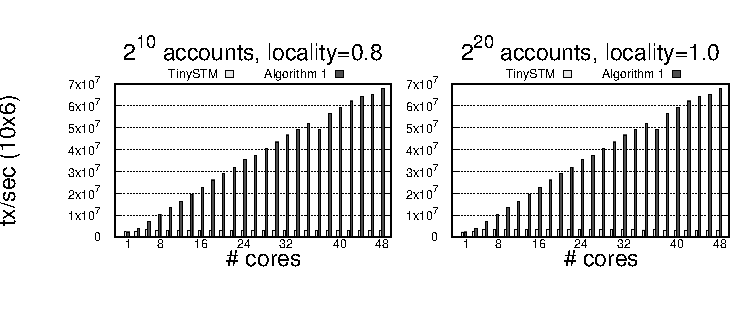
\includegraphics[scale = 1.0]{results/intset/bank.pdf}
	\caption{Bank Benchmark. Left: 80\% locality. Right: 100\% locality.\label{fig:benchmarking:bank}}
\end{figure}

\begin{figure}[!t]
	\centering
	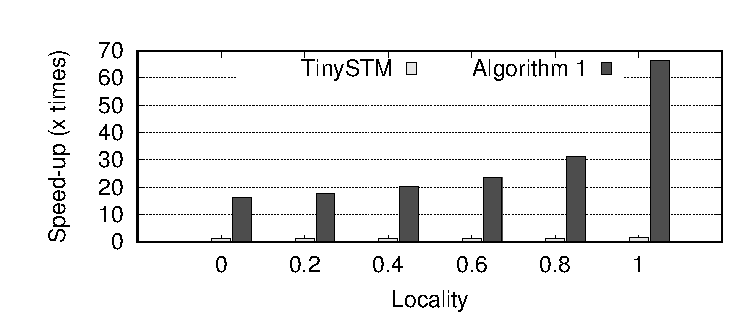
\includegraphics[scale = 0.8]{results/bank-speedup/bank-speedup.pdf}
	\caption{Bank Benchmark. Speed-up of our algorithm for different locality levels. In this experiment, we always use 48 cores.\label{fig:benchmarking:bank:speedup}}
\end{figure}


\subsection{Benchmark: Linked-list}

The linked-list benchmark consists in modifying a sorted linked list concurrently. 
Each thread randomly adds or removes a node from the list. 
We run this benchmark with a range of 512 (meaning that each thread randomly adds/removes a value comprised between -255 and +256) and a linked list initialized with 256 values.
Figure~\ref{fig:benchmarking:llrb}(left) reports our results.

The results show that the global clock outperforms our implementation. 
This is due to the high contention in this application that causes our optimistic algorithm to abort \ft{that's not the right verb} many transactions.

\begin{figure}[!t]
	\centering
	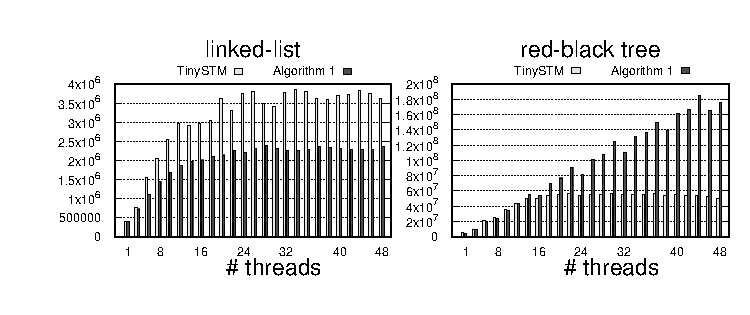
\includegraphics[scale = 1.0]{results/intset/ll-rb.pdf}
	\caption{Linked-list (left) and Red-Black tree (right) benchmarks.\label{fig:benchmarking:llrb}}
\end{figure}

\subsection{Reb-black tree}

The red-black tree benchmark is similar to the linked-list benchmark except that the values are stored in a self-balancing binary search tree. 
We run this benchmark with a range of $10^7$ values, and a binary tree initialized with $10^5$ values.
Figure~\ref{fig:benchmarking:llrb}(right) reports our results.

When using the global clock, the performance of this application improves linearly up to 12 threads. 
It then stalls to approximately 50 millions transactions per second.

On this application, our implementation scales linearly as the number of threads grows. 
It achieves 176 millions transactions per second with 48 threads.
%
In this benchmark, the likelyhood of a concurrent transaction is very low because of the high number of values in the tree. However,\ft{explain why the global clock performs poorly}.
%
